\setchapterpreamble[u]{\margintoc}
\chapter{Coordenadas Curvilíneas Ortogonales}
\labch{coordenadas_curvilineas_ortogonales}

Los sistemas de coordenadas curvilíneas ortogonales hacen referencia a puntos en el espacio determinados por el corte de tres superficies, tales que, los vectores unitarios tangentes a cada curva de la intersección de dos de ellos son ortogonales entre sí.

Como ejemplo, revisemos que ocurre en las coordenadas cartesianas. Allí, cada punto espacial es determinado por la intersección de tres planos mutuamente ortogonales entre sí y que adicionalmente los tres vectores unitarios $\hat{i}, \hat{j}, \hat{k}$ permanecerán siendo los mismos mediante una operación de traslación de ellos al punto en consideración.

\begin{center}
  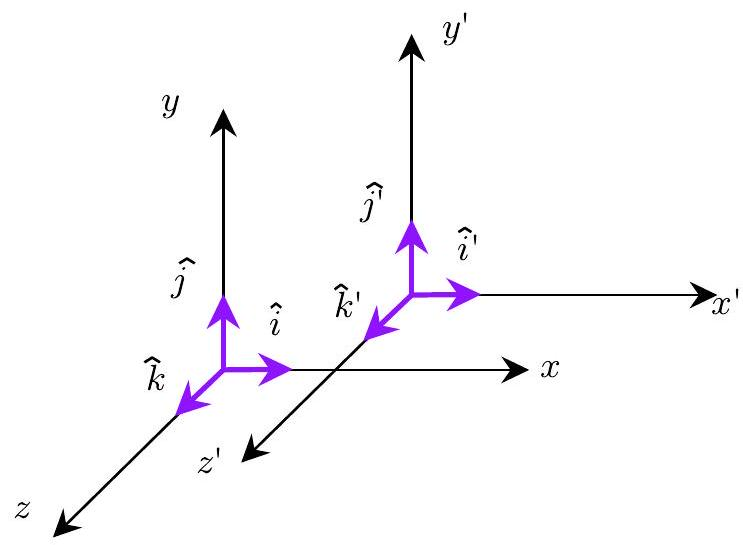
\includegraphics[max width=\textwidth]{sistemas_coordenados.jpg}
\end{center}

De tal forma que $\hat{i}=\hat{i}^{\prime}, \hat{j}=\hat{j}^{\prime}, \hat{k}=\hat{k}^{\prime}$

Miremos ahora que sucede en coordenadas cilíndricas. En este caso, las tres superficies que se intersectan son:

\begin{itemize}
  \item Un cilindro, un plano y un semiplano, De esta manera las tres nuevas variables serán: $\rho$ el radio del cilindro, $\theta$ el ángulo de apertura del semiplano y $z$ la posición del plano. Observemos esto en la siguiente figura:
\end{itemize}

\begin{center}
  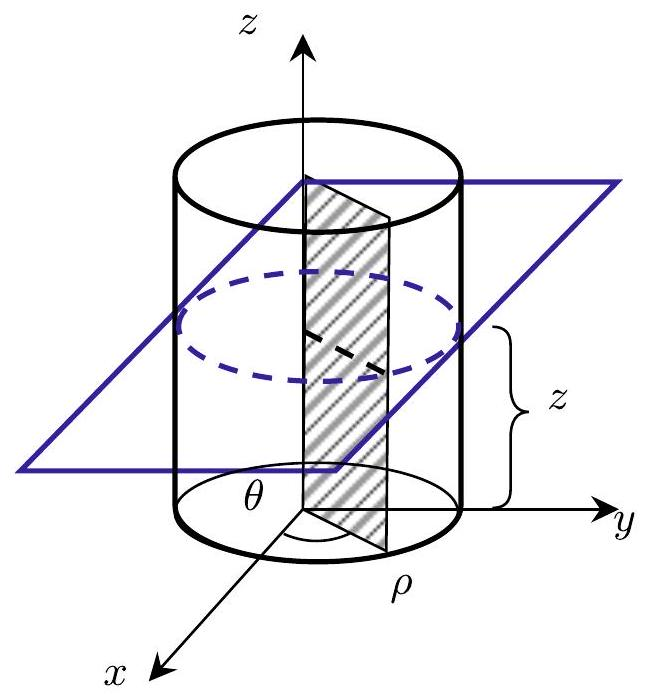
\includegraphics[max width=\textwidth]{coord_cilindricas.jpg}
\end{center}

Como se evidencia en la figura, la curva producto del corte entre el cilindro y el semiplano es una línea recta vertical, que determinará la coordenada $z$; la curva determinada por el corte del semiplano y el plano, determinará una semirecta que será $\rho$ y por último el corte entre el plano y el cilindro, será una circunferencia, que determinará $\theta$. De esta forma los tres vectores unitarios ortogonales entre sí y tangentes a estas curvas, serán:

$\hat{e}_{\rho}:$ vector tangente a la semirecta

$\hat{e}_{\theta}$ : vector tangente a la circunferencia

$\hat{e}_{z}$ : vector tangente a la recta vertical

Ellos forman entre sí un conjunto de mano derecha, por lo tanto

$$
\hat{e}_{\rho}=\hat{e}_{\theta} \times \hat{e}_{z}, \quad \hat{e}_{z}=\hat{e}_{\rho} \times \hat{e}_{\theta}, \quad \widehat{e}_{\theta}=\hat{e}_{z} \times \hat{e}_{\rho} .
$$

Adicionalmente, la propiedad de ortogonalidad la evidencio como:

$$
\widehat{e}_{\rho} \cdot \widehat{e}_{\theta}=\widehat{e}_{\rho} \cdot \widehat{e}_{z}=\widehat{e}_{\theta} \cdot \hat{e}_{z}=0
$$

Por último, como ejemplo, revisemos el caso de las coordenadas esféricas. En este caso las superficies que se intersectan son: una esfera, un semiplano y un tronco de cono.

Las respectivas curvas que se producen son:

\begin{itemize}
  \item De la intersección del tronco de cono y la esfera, una circunferencia.

  \item Del cono y el semiplano una semirecta.

  \item Del semiplano y la esfera, una semicircunferencia.

\end{itemize}

Lo que determina tres vectores unitarios ortogonales

$\hat{e}_{r}$ : vector tangente a la semirecta

$\hat{e}_{\theta}$ : vector tangente a la semicircunferencia

$\hat{e}_{\varphi}:$ vector tangente a la circunferencia

y las tres variables $r, \theta, \varphi$.

De nuevo este conjunto de vectores unitarios forman un conjunto de mano derecha, por lo tanto:

$$
\widehat{e}_{r}=\widehat{e}_{\theta} \times \hat{e}_{\varphi}, \hat{e}_{\varphi}=\widehat{e}_{r} \times \widehat{e}_{\theta}, \widehat{e}_{\theta}=\hat{e}_{\varphi} \times \hat{e}_{r}
$$

Debe notarse muy especialmente que en cualquier sistema de coordenadas curvilíneas ortogonales que no sea el cartesiano, la dirección de los vectores unitarios cambia punto a punto. Este hecho es importante, pues, mientras los vectores $\hat{i}, \hat{j}, \hat{k}$ no varían punto a punto, los otros si lo harán. Para los dos últimos casos mencionados debe tenerse en cuenta que las respectivas transformaciones de coordenadas entre estos sistemas y el cartesiano, son:

\begin{center}
\begin{tabular}{|l|l|}
\hline
Cilíndricas & Esféricas \\
\hline
\end{tabular}
\end{center}

$$
x=\rho \cos \theta, y=\rho \sin \theta, z
$$

$$
\begin{aligned}
& x=r \sin \theta \cos \varphi \\
& y=r \sin \theta \sin \varphi \\
& z=r \cos \theta
\end{aligned}
$$

Dentro del espacio Euclideo, se reconocen los siguientes sistemas de coordenadas curvilíneas ortogonales

\begin{center}
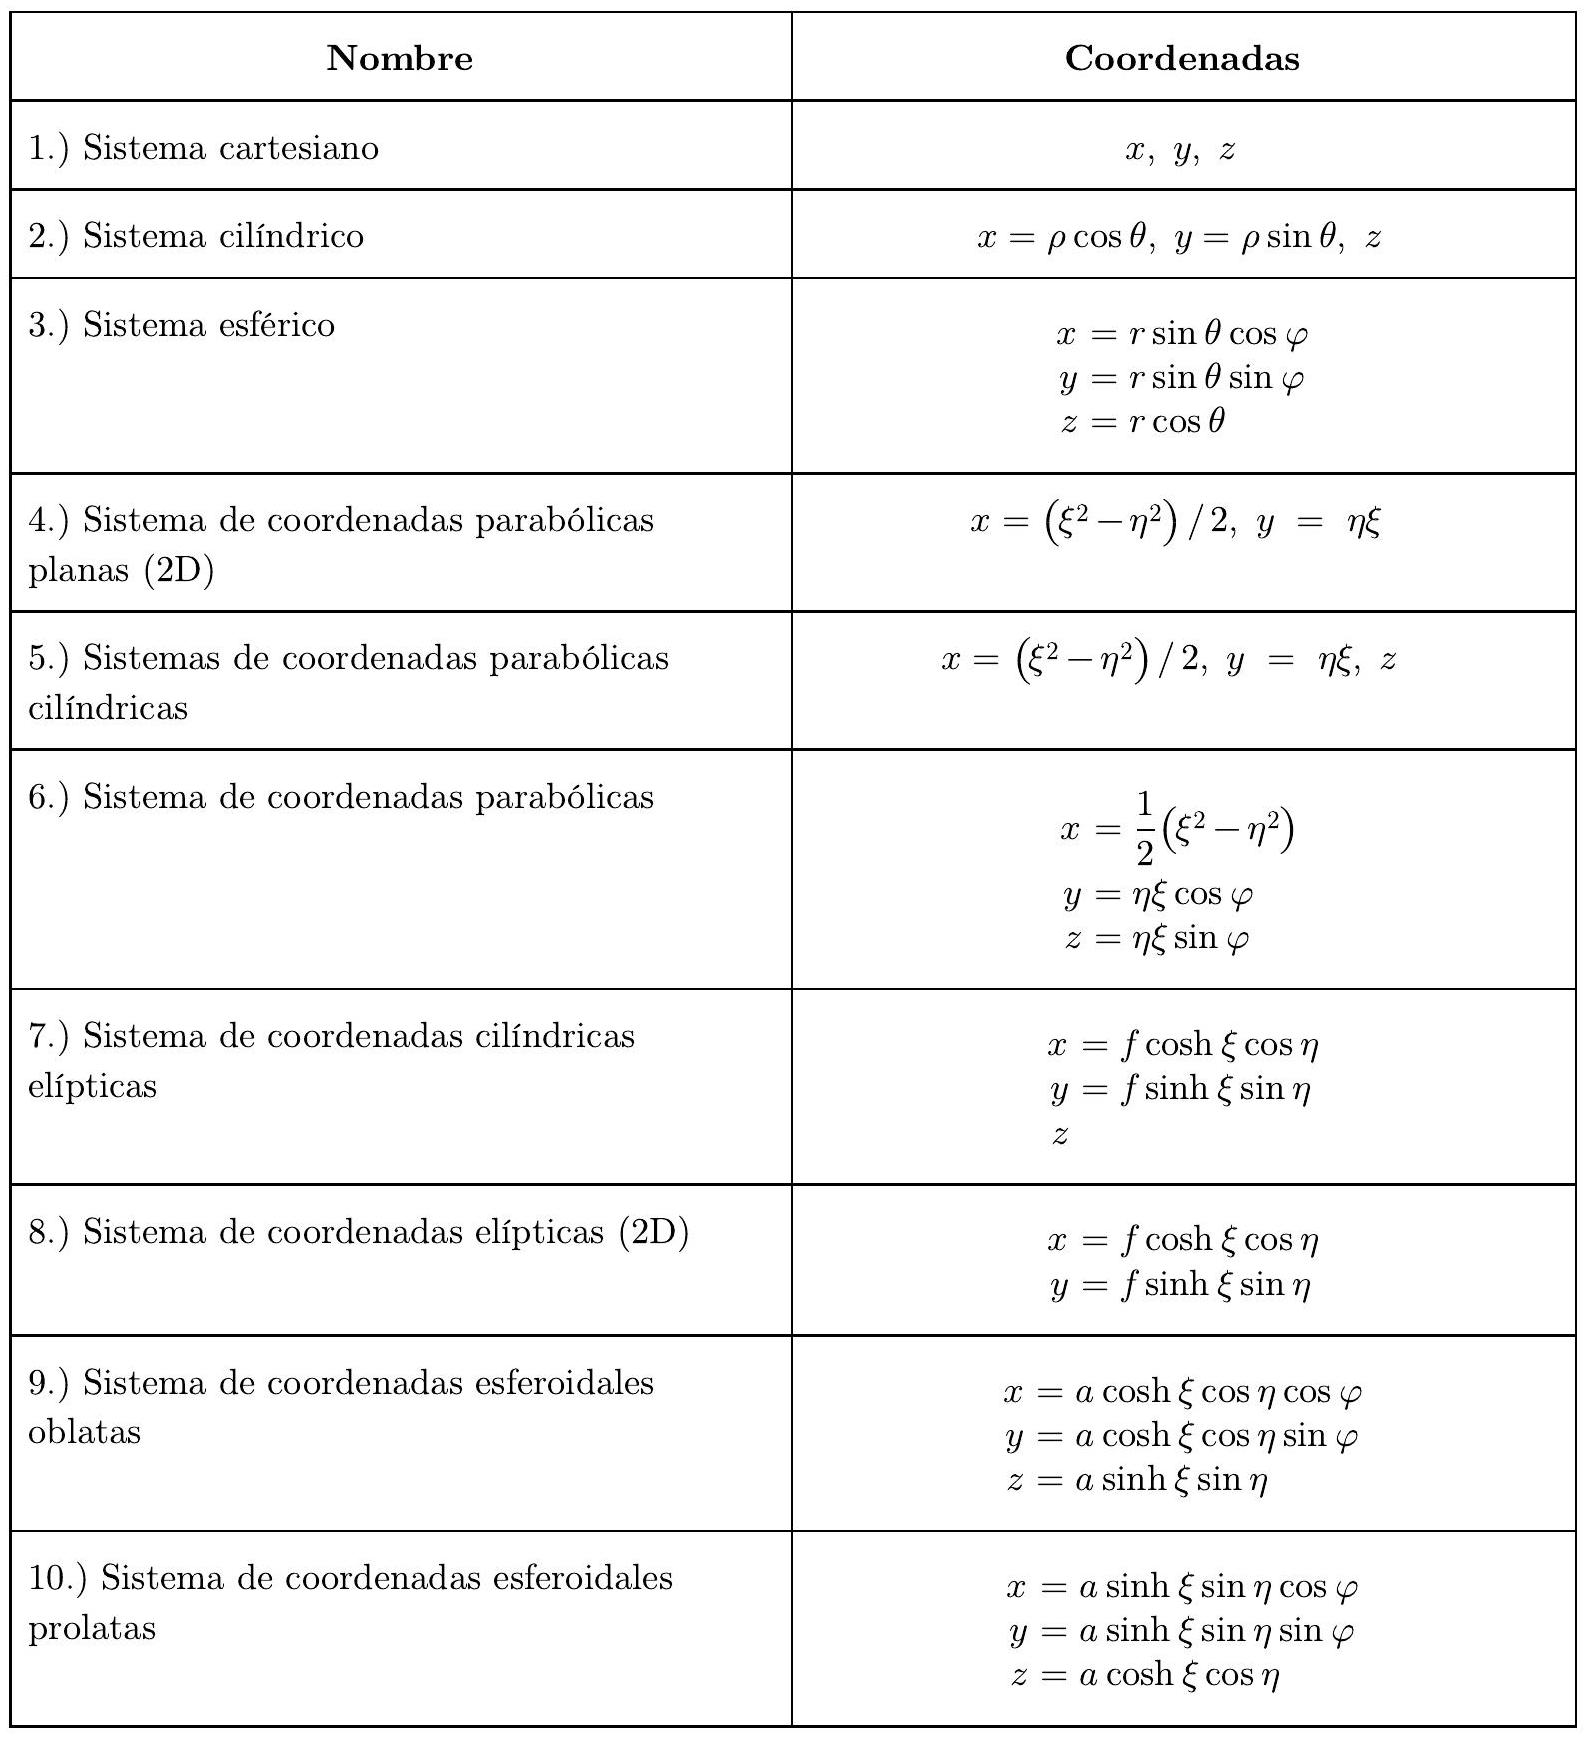
\includegraphics[max width=\textwidth]{tabla_sistemas_coordenados.jpg}
\end{center}

\begin{center}
\begin{tabular}{|l|l|}
\hline
11.) Sistema de coordenadas bipolares & $x=\frac{a \sinh \eta}{\cosh \eta-\cos \xi}$ \\
 & $y=\frac{a \sin \xi}{\cosh \eta-\cos \xi}$ \\
 & $z$ \\
\hline
12.) Sistema de coordenadas toroidales & $x=\frac{a \sinh \eta \cos \varphi}{\cosh \eta-\cos \xi}$ \\
 & $y=\frac{a \sinh \eta \sin \varphi}{\cosh \eta-\cos \xi}$ \\
 & $z=\frac{a \sin \xi}{\cosh \eta-\cos \xi}$ \\
\hline
13.) Sistema de coordenadas biesféricas & $y=\frac{a \sin \xi \cos \varphi}{\cosh \eta-\cos \xi}$ \\
 & $y=\frac{a \sin \xi \sin \varphi}{\cosh \eta-\cos \xi}$ \\
 & $z=\frac{a \sinh \eta}{\cosh \eta-\cos \xi}$ \\
\hline
\end{tabular}
\end{center}

Cada sistema coordenado tendrá un dominio para cada una de sus variables, de modo que queden cubiertos todos los puntos del plano o el espacio según sea la situación.

Consideremos ahora la siguiente situación general, si $x=x\left(u_{1}, u_{2}, u_{3}\right), y=y\left(u_{1}, u_{2}, u_{3}\right)$ y $z=z\left(u_{1}, u_{2}, u_{3}\right)$, del cálculo diferencial

$$
\begin{aligned}
& d x=\frac{\partial x\left(u_{1}, u_{2}, u_{3}\right)}{\partial u_{1}} d u_{1}+\frac{\partial x\left(u_{1}, u_{2}, u_{3}\right)}{\partial u_{2}} d u_{2}+\frac{\partial x\left(u_{1}, u_{2}, u_{3}\right)}{\partial u_{3}} d u_{3} \\
& d y=\frac{\partial y\left(u_{1}, u_{2}, u_{3}\right)}{\partial u_{1}} d u_{1}+\frac{\partial y\left(u_{1}, u_{2}, u_{3}\right)}{\partial u_{2}} d u_{2}+\frac{\partial y\left(u_{1}, u_{2}, u_{3}\right)}{\partial u_{3}} d u_{3} \\
& d z=\frac{\partial z\left(u_{1}, u_{2}, u_{3}\right)}{\partial u_{1}} d u_{1}+\frac{\partial z\left(u_{1}, u_{2}, u_{3}\right)}{\partial u_{2}} d u_{2}+\frac{\partial z\left(u_{1}, u_{2}, u_{3}\right)}{\partial u_{3}} d u_{3}
\end{aligned}
$$

De tal manera,

$$
\begin{aligned}
d \vec{r} & =\frac{\partial \vec{r}}{\partial u_{1}} d u_{1}+\frac{\partial \vec{r}}{\partial u_{2}} d u_{2}+\frac{\partial \vec{r}}{\partial u_{3}} d u_{3} \\
& =\sum_{i=1}^{3} \frac{\partial \vec{r}}{\partial u_{i}} d u_{i}
\end{aligned}
$$

Si se propone que: $\frac{\partial \vec{r}}{\partial u_{i}}=h_{i} \hat{e}_{i}$, entendiendo que la derivada de $\vec{r}$ se escribe en la base de vectores $\left\{\widehat{e}_{i}\right\}$ unitarios. De ahí desprendemos,

$$
h_{i}=\left|\frac{\partial \vec{r}}{\partial u_{i}}\right| \quad \hat{e}_{i}=\frac{1}{h_{i}} \frac{\partial \vec{r}}{\partial u_{i}}
$$

La constante de proporcionalidad $h_{i}$ recibe el nombre de factor de escala.

\section{Ejemplos:}
Encuentre los factores de escala y los vectores unitarios en coordenadas cilíndricas y esféricas.

Escribamos a $\vec{r}$ en coordenadas cartesianas

$$
\vec{r}=x \hat{i}+y \hat{j}+z \hat{k}
$$

Con la transformación: $x=\rho \cos \theta, y=\rho \sin \theta, z$

$$
\begin{aligned}
& \vec{r}=\rho \cos \theta \hat{i}+\rho \sin \theta \hat{j}+z \hat{k} \\
h_{\rho} & =\left|\frac{\partial}{\partial \rho}\{\rho \cos \theta \hat{i}+\rho \sin \theta \hat{j}+z \hat{k}\}\right| \\
= & |\cos \theta \hat{i}+\sin \theta \hat{j}| \\
= & \sqrt{\sin ^{2} \theta+\cos ^{2} \theta} \\
h_{\rho} & =1 \\
h_{\theta} & =\left|\frac{\partial}{\partial \theta}\{\rho \cos \theta \hat{i}+\rho \sin \theta \hat{j}+z \hat{k}\}\right| \\
= & \mid-\rho \sin \theta \hat{i}+\rho \cos \theta \hat{j}\rceil \\
& =\sqrt{\rho^{2}\left(\sin 2 \theta+\cos ^{2} \theta\right)} \\
h_{\theta} & =\rho \\
h_{z}= & \left|\frac{\partial}{\partial z}\{\rho \cos \theta \hat{i}+\rho \sin \theta \hat{j}+z \hat{k}\}\right| \\
& =|1 \hat{k}| \\
h_{z} & =1
\end{aligned}
$$

De esta manera los factores de escala en coordenadas cilíndricas, son:

$$
\left(h_{\rho}, h_{\theta}, h_{z}\right)=(1, \rho, 1)
$$

De acá los vectores unitarios, son: $\left(\widehat{e}_{i}=\frac{1}{h_{i}} \frac{\partial \vec{r}}{\partial u_{i}}\right)$

$$
\begin{aligned}
\widehat{e}_{\rho} & =\frac{1}{h_{\rho}} \frac{\partial \vec{r}}{\partial \rho} \\
& =\frac{\partial \vec{r}}{\partial \rho} \quad\left(\text { ya que } h_{\rho}=1\right) \\
& =\frac{\partial}{\partial \rho}\{\rho \cos \theta \hat{i}+\rho \sin \theta \hat{j}+z \hat{k}\} \\
\hat{e}_{\rho} & =\cos \theta \hat{i}+\sin \theta \hat{j}
\end{aligned}
$$

$$
\begin{aligned}
\hat{e}_{\theta} & =\frac{1}{h_{\theta}} \frac{\partial \vec{r}}{\partial \theta} \\
& =\frac{1}{\rho} \frac{\partial}{\partial \theta}\{\rho \cos \theta \hat{i}+\rho \sin \theta \hat{j}+z \hat{k}\} \\
\hat{e}_{\theta} & =-\sin \theta \hat{i}+\cos \theta \hat{j} \\
\widehat{e}_{z} & =\frac{1}{h_{z}} \frac{\partial \vec{r}}{\partial z} \\
& =\frac{\partial \vec{r}}{\partial z}\left(\text { ya que } h_{z}=1\right) \\
& =\frac{\partial}{\partial z}\{\rho \cos \theta \hat{i}+\rho \sin \theta \hat{j}+z \hat{k}\} \\
\hat{e}_{z} & =\hat{k}
\end{aligned}
$$

Por lo tanto

$$
\left\{\widehat{e}_{\rho}, \hat{e}_{\theta}, \hat{e}_{z}\right\}=\{\cos \theta \hat{i}+\sin \theta \hat{j},-\sin \theta \hat{i}+\cos \theta \hat{j}, \hat{k}\}
$$

De donde podemos constatar que:

$$
\begin{aligned}
\widehat{e}_{\rho} \cdot \hat{e}_{\theta} & =(\cos \theta \hat{i}+\sin \theta \hat{j}) \cdot(-\sin \theta \hat{i}+\cos \theta \hat{j}) \\
& =-\sin \theta \cos \theta+\sin \theta \cos \theta \\
& =0 \\
\hat{e}_{\rho} \cdot \widehat{e}_{z} & =(\cos \theta \hat{i}+\sin \theta \hat{j}) \cdot(\hat{k}) \\
& =0 \\
\widehat{e}_{\theta} \cdot \hat{e}_{z} & =(-\sin \theta \hat{i}+\cos \theta \hat{j}) \cdot(\hat{k}) \\
& =0
\end{aligned}
$$

$\mathrm{Y}$

$$
\begin{aligned}
& \hat{e}_{\rho} \cdot \hat{e}_{\rho}=(\cos \theta \hat{i}+\sin \theta \hat{j}) \cdot(\cos \theta \hat{i}+\sin \theta \hat{j}) \\
& =\cos ^{2} \theta+\sin ^{2} \theta \\
& =1 \\
& \widehat{e}_{\theta} \cdot \hat{e}_{\theta}=(-\sin \theta \hat{i}+\cos \theta \hat{j}) \cdot(-\sin \theta \hat{i}+\cos \theta \hat{j}) \\
& =\sin ^{2} \theta+\cos ^{2} \theta \\
& =1 \\
& \hat{e}_{z} \cdot \hat{e}_{z}=(\hat{k}) \cdot(\widehat{k}) \\
& =1
\end{aligned}
$$

Lo cual muestra que se tiene una base de vectores unitarios y ortogonales $\left(\hat{e}_{\rho}, \hat{e}_{\theta}, \hat{e}_{z}\right)$. También se puede verificar que es un sistema de mano derecha. Verifiquemos que $\widehat{e}_{\rho}=\hat{e}_{\theta} \times \hat{e}_{z}$

$$
\begin{aligned}
\hat{e}_{\theta} \times \widehat{e}_{z} & =\left|\begin{array}{ccc}
\hat{i} & \hat{j} & \hat{k} \\
-\sin \theta & \cos \theta & 0 \\
0 & 0 & 1
\end{array}\right| \\
& =(\cos \theta-0) \hat{i}-(-\sin \theta-0) \hat{j}+(0-0) \hat{k} \\
& =\cos \theta \hat{i}+\sin \theta \hat{j}
\end{aligned}
$$

Como $\hat{e}_{\rho}=\cos \theta \hat{i}+\sin \theta \hat{j}$, entonces

$$
\hat{e}_{\rho}=\hat{e}_{\theta} \times \hat{e}_{z}
$$

De manera análoga:

$$
\hat{e}_{\theta}=\widehat{e}_{z} \times \widehat{e}_{\rho}
$$

Calculemos:

$$
\begin{aligned}
\hat{e}_{z} \times \hat{e}_{\rho} & =\left|\begin{array}{ccc}
\hat{i} & \hat{j} & \hat{k} \\
0 & 0 & 1 \\
\cos \theta & \sin \theta & 0
\end{array}\right| \\
& =(0-\sin \theta) \hat{i}-(0-\cos \theta) \hat{j}+(0-0) \hat{k} \\
& =-\sin \theta \hat{i}+\cos \theta \hat{j}
\end{aligned}
$$

Como $\hat{e}_{\theta}=-\sin \theta \hat{i}+\cos \theta \hat{j}$, entonces se ha verificado que: $\hat{e}_{\theta}=\hat{e}_{z} \times \hat{e}_{\rho}$.

Finalmente verifiquemos que: $\widehat{e}_{z}=\widehat{e}_{\rho} \times \widehat{e}_{\theta}$

$$
\begin{aligned}
\widehat{e}_{\rho} \times \widehat{e}_{\theta} & =\left|\begin{array}{ccc}
\hat{i} & \hat{j} & \hat{k} \\
\cos \theta & \sin \theta & 0 \\
-\sin \theta & \cos \theta & 0
\end{array}\right| \\
& =(0-0) \hat{i}-(0-0) \hat{j}+\left(\cos ^{2} \theta+\sin ^{2} \theta\right) \hat{k} \\
& =\widehat{k}
\end{aligned}
$$

Por lo tanto $\hat{e}_{z}=\hat{e}_{\rho} \times \hat{e}_{\theta}$

\section{Tarea:}
\begin{itemize}
  \item Realizar todo lo anterior para las coordenadas esféricas, es decir, encontrar factores de escala, vectores unitarios, probar su ortogonalidad, unitariedad y regla de la mano derecha.

  \item Tomar las coordenadas esferoidales oblatas y hacer todo lo anterior.

\end{itemize}


Clase 2

Como ha sido mostrado en la clase anterior la transformación de coordenadas y de vectores unitarios en el cilíndrico corresponde a:

$$
x=\rho \cos \theta, y=\rho \sin \theta, z
$$

$\mathrm{Y}$ los vectores unitarios como:

$$
\begin{aligned}
& \hat{e}_{\rho}=\cos \theta \hat{i}+\sin \theta \hat{j} \\
& \widehat{e}_{\theta}=-\sin \theta \hat{i}+\cos \theta \hat{j} \\
& \widehat{e}_{z}=\widehat{k}
\end{aligned}
$$

La relación entre los vectores unitarios del sistema cilíndrico y del sistema cartesiano pueden escribirse matricialmente de la siguiente forma:

$$
\left(\begin{array}{l}
\hat{e}_{\rho} \\
\hat{e}_{\theta} \\
\hat{e}_{z}
\end{array}\right)=\left(\begin{array}{ccc}
\cos \theta & \sin \theta & 0 \\
-\sin \theta & \cos \theta & 0 \\
0 & 0 & 1
\end{array}\right)\left(\begin{array}{l}
\hat{i} \\
\hat{j} \\
\hat{k}
\end{array}\right)
$$

La matriz de transformación es unitaria y por esto $\mathbb{M}^{T}=\mathbb{M}^{-1}$, de esta manera si se desean obtener $\hat{i}, \hat{j}, \hat{k}$ en términos de $\hat{e}_{\rho}, \widehat{e}_{\theta}, \hat{e}_{z}$ debe despejarse como:

$$
\left(\begin{array}{c}
\hat{i} \\
\hat{j} \\
\hat{k}
\end{array}\right)=\left(\begin{array}{ccc}
\cos \theta & \sin \theta & 0 \\
-\sin \theta & \cos \theta & 0 \\
0 & 0 & 1
\end{array}\right)^{-1}\left(\begin{array}{l}
\hat{e}_{\rho} \\
\hat{e}_{\theta} \\
\hat{e}_{z}
\end{array}\right)
$$

De este modo

$$
\left(\begin{array}{l}
\hat{i} \\
\hat{j} \\
\hat{k}
\end{array}\right)=\left(\begin{array}{ccc}
\cos \theta & -\sin \theta & 0 \\
\sin \theta & \cos \theta & 0 \\
0 & 0 & 1
\end{array}\right)\left(\begin{array}{l}
\hat{e}_{\rho} \\
\hat{e}_{\theta} \\
\hat{e}_{z}
\end{array}\right)
$$

Siendo así que:

$$
\begin{aligned}
& \hat{i}=\cos \theta \widehat{e}_{\rho}-\sin \theta \widehat{e}_{\theta} \\
& \hat{j}=\sin \theta \widehat{e}_{\rho}+\cos \theta \widehat{e}_{\theta} \\
& \hat{k}=\hat{e}_{z}
\end{aligned}
$$

En general podríamos escribir lo anterior como:

$$
\left(\begin{array}{l}
\hat{e}_{1} \\
\hat{e}_{2} \\
\hat{e}_{3}
\end{array}\right)=\left(\begin{array}{cccc}
\frac{1}{h_{1}} \frac{\partial x}{\partial u_{1}} & \frac{1}{h_{1}} \frac{\partial y}{\partial u_{1}} & \frac{1}{h_{1}} \frac{\partial z}{\partial u_{1}} \\
\frac{1}{h_{2}} \frac{\partial x}{\partial u_{2}} & \frac{1}{h_{2}} \frac{\partial y}{\partial u_{2}} & \frac{1}{h_{2}} \frac{\partial z}{\partial u_{2}} \\
\frac{1}{h_{3}} \frac{\partial x}{\partial u_{3}} & \frac{1}{h_{3}} \frac{\partial y}{\partial u_{3}} & \frac{1}{h_{3}} \frac{\partial z}{\partial u_{3}}
\end{array}\right)\left(\begin{array}{l}
\hat{i} \\
\hat{j} \\
\hat{k}
\end{array}\right)
$$

Y por lo tanto

$$
\left(\begin{array}{l}
\hat{i} \\
\hat{j} \\
\hat{k}
\end{array}\right)=\left(\begin{array}{cccc}
\frac{1}{h_{1}} \frac{\partial x}{\partial u_{1}} & \frac{1}{h_{2}} \frac{\partial x}{\partial u_{2}} & \frac{1}{h_{3}} \frac{\partial x}{\partial u_{3}} \\
\frac{1}{h_{1}} \frac{\partial y}{\partial u_{1}} & \frac{1}{h_{2}} \frac{\partial y}{\partial u_{2}} & \frac{1}{h_{3}} \frac{\partial y}{\partial u_{3}} \\
\frac{1}{h_{1}} \frac{\partial z}{\partial u_{1}} & \frac{1}{h_{2}} \frac{\partial z}{\partial u_{2}} & \frac{1}{h_{3}} \frac{\partial z}{\partial u_{3}}
\end{array}\right)\left(\begin{array}{l}
\hat{e}_{1} \\
\hat{e}_{2} \\
\hat{e}_{3}
\end{array}\right)
$$

Ejemplo: Sea el vector $\vec{B}=\left(B_{x}, B_{y}, B_{z}\right)=3 \hat{i}+7 \hat{j}+5 \hat{k} \quad$ en coordenadas cartesianas. Represente dicho vector en coordenadas cilíndricas, es decir, encuentre $\left(B_{\rho}, B_{\theta}, B_{z}\right)$

\subsection{Solución:}
$$
\begin{aligned}
\vec{B} & =3\left(\cos \theta \widehat{e}_{\rho}-\sin \theta \widehat{e}_{\theta}\right)+7\left(\sin \theta \widehat{e}_{\rho}+\cos \theta \widehat{e}_{\theta}\right)+5 \widehat{e}_{z} \\
& =(3 \cos \theta+7 \sin \theta) \widehat{e}_{\rho}+(-3 \sin \theta+7 \cos \theta) \widehat{e}_{\theta}+5 \widehat{e}_{z}
\end{aligned}
$$

Luego, $B_{\rho}=3 \cos \theta+7 \sin \theta, B_{\theta}=-3 \sin \theta+7 \cos \theta, B_{z}=5$

Ejercicio: Haga todo lo anterior ya no para cilíndricas sino para esféricas

\subsection{Elementos de Línea, Superficie y Volumen}
Definiremos

$$
\begin{aligned}
d \vec{r} & =\sum_{i=1}^{3} h_{i} \widehat{e}_{i} d u_{i} \\
& =\sum_{i=1}^{3} d \vec{l}_{i}
\end{aligned}
$$

Por lo tanto

$$
d \vec{l}_{i}=h_{i} \widehat{e}_{i} d u_{i}
$$

En general estos elementos diferenciales de línea orientados, corresponderán a longitudes de segmentos de líneas rectas o de arcos de curvas. Así pues, en coordenadas cilíndricas:

$$
\begin{array}{rlrl}
d \vec{l}_{\rho} & =h_{\rho} \widehat{e}_{\rho} d \rho & \\
& =\widehat{\rho} d \rho & & \text { (Longitud } d \rho \text { orientada en dirección de } \widehat{\rho}) \\
d \vec{l}_{\theta} & =h_{\theta} \widehat{e}_{\theta} d \theta & \\
& =\rho \hat{\theta} d \theta & & \\
d \vec{l}_{z} & =h_{z} \widehat{e}_{z} d z & \text { ( Longitud del arco } \rho d \theta \text { en la dirección de } \hat{\theta}) \\
& =\hat{k} d z \quad & \quad
\end{array}
$$

Hagamos lo correspondiente para las coordenadas esféricas

$$
\begin{aligned}
d \vec{l}_{r} & =h_{r} \widehat{e}_{r} d r \\
& =\widehat{r} d r \\
d \vec{l}_{\theta} & =h_{\theta} \widehat{e}_{\theta} d \theta \\
& =r \widehat{\theta} d \theta \\
d \vec{l}_{\varphi} & =h_{\varphi} \widehat{e}_{\varphi} d \varphi \\
& =r \sin \theta \widehat{\varphi} d \varphi
\end{aligned}
$$

( Longitud $d r$ orientada en dirección $\widehat{r}$ )

( Longitud del arco $r d \theta$ orientado en la dirección $\widehat{\theta}$ )

( Longitud del arco $r \sin \theta$ orientado en la dirección de $\widehat{\varphi}$ )

Recuerde en cada caso reflexionar geométricamente a que corresponde cada longitud y cada arco.

\subsection{Ejercicio:}
Encuentre los elementos de línea en las coordenadas bipolares

A partir de los elementos diferenciales de línea definidos anteriormente y con uso del cálculo vectorial. definiremos a través del producto cruz y la regla de la mano derecha el elemento diferencial de superficie.

\begin{center}
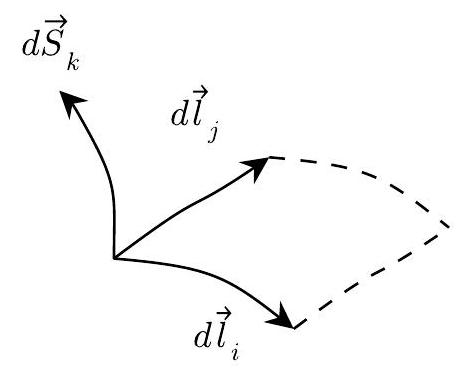
\includegraphics[max width=\textwidth]{2023_01_15_4065f1f4fc9993406c61g-3}
\end{center}

Con $d \vec{S}_{k}=d \vec{l}_{i} \times d \vec{l}_{j}$ y $i, j, k$ siguiendo la regla de la mano derecha.

De esto se desprende que en un sistema de coordenadas curvilíneas ortogonales, se definen tres diferenciales de superficie básicos. Por ejemplo en coordenadas cilíndricas tenemos:

$$
\begin{aligned}
d \vec{S}_{\rho} & =d \vec{l}_{\theta} \times d \vec{l}_{z} \\
& =\left(h_{\theta} d \theta\right)\left(h_{z} d z\right) \hat{\theta} \times \widehat{k} \\
& =\rho d \theta d z \widehat{\rho}
\end{aligned}
$$

Observemos que dicho elemento tiene unidades de área y que corresponde al producto del arco $\rho d \theta$ por $d z$, es decir, un área en la superficie del cilindro, además orientada perpendicularmente a la superficie del mismo

$$
\begin{aligned}
d \vec{S}_{\theta} & =d \vec{l}_{z} \times d \vec{l}_{\rho} \\
& =\left(h_{z} d z\right)\left(h_{\rho} d \rho\right) \hat{k} \times \hat{\rho} \\
& =d \rho d z \hat{\theta}
\end{aligned}
$$

En este caso es el área en el semiplano y está orientada en dirección perpendicular determinada por $\hat{\theta}$. Finalmente

$$
\begin{aligned}
d \vec{S}_{z} & =d \vec{l}_{\rho} \times d \vec{l}_{\theta} \\
& =\left(h_{\rho} d \rho\right)\left(h_{\theta} d \theta\right) \hat{\rho} \times \widehat{\theta} \\
& =\rho d \rho d \theta \hat{k}
\end{aligned}
$$

En este caso el área es definida en el plano y la dirección es en $\hat{k}$, claramente perpendicular al mismo. Revisemos este concepto en coordenadas esféricas:

$$
\begin{aligned}
d \vec{S}_{r} & =d \vec{l}_{\theta} \times d \vec{l}_{\varphi} \\
& =\left(h_{\theta} d_{\theta}\right)\left(h_{\varphi} d \varphi\right) \widehat{\theta} \times \widehat{\varphi} \\
& =r^{2} \sin \theta d \theta d \varphi \widehat{r}
\end{aligned}
$$

En este caso será un elemento diferencial de área en la superficie de la esfera, con dirección en $\widehat{r}$. (Producto de los arcos en $\theta$ y $\varphi$ )

$$
\begin{aligned}
d \vec{S}_{\theta} & =d \vec{l}_{\varphi} \times d \vec{l}_{r} \\
& =\left(h_{\varphi} d \varphi\right)\left(h_{r} d r\right) \widehat{\varphi} \times \widehat{r} \\
& =r \sin \theta d r d \varphi \widehat{\theta}
\end{aligned}
$$

Este elemento diferencial corresponde a un área sobre el tronco de cono y dirección determinada por $\hat{\theta}$.

$$
\begin{aligned}
d \vec{S}_{\varphi} & =d \vec{l}_{r} \times d \vec{l}_{\theta} \\
& =\left(h_{r} d r\right)\left(h_{\theta} d \theta\right) \widehat{r} \times \widehat{\theta} \\
& =r d r d \theta \widehat{\varphi}
\end{aligned}
$$

Este elemento diferencial corresponde a un área en el semiplano, con un vector perpendicular al área $\widehat{\varphi}$.

Ejercicio: Encuentre los elementos de área en el caso de coordenadas parabólicas cilíndricas.

Finalmente, el diferencial de volumen lo calcularemos como el volumen de un paralelepípedo, así:

$$
d V=d \vec{l}_{1} \cdot\left(d \vec{l}_{2} \times d \vec{l}_{3}\right)
$$

o cualquier permutación cíclica de los índices 1,2,3 - Para coordenadas cilíndricas:

$$
\begin{aligned}
d V & =d \vec{l}_{\rho} \cdot\left(d \vec{l}_{\theta} \times d \vec{l}_{z}\right) \\
& =\left(h_{\rho} d \rho\right)\left(h_{\theta} d \theta\right)\left(h_{z} d z\right) \widehat{\rho} \cdot(\widehat{\theta} \times \widehat{k}) \\
& =\rho d \rho d \theta d z \widehat{\rho} \cdot \widehat{\rho} \\
d V & =\rho d \rho d \theta d z
\end{aligned}
$$

\begin{itemize}
  \item Para coordenadas esféricas:
\end{itemize}

$$
\begin{aligned}
d V & =d \vec{l}_{r} \cdot\left(d \vec{l}_{\theta} \times d \vec{l}_{\varphi}\right) \\
& =\left(h_{r} d r\right)\left(h_{\theta} d \theta\right)\left(h_{\varphi} d \varphi\right) \widehat{r} \cdot(\widehat{\theta} \times \widehat{\varphi}) \\
& =r^{2} \sin \theta d r d \theta d \varphi \widehat{r} \cdot \widehat{r} \\
d V & =r^{2} \sin \theta d r d \theta d \varphi
\end{aligned}
$$

En general, $d V=h_{1} h_{2} h_{3} d u_{1} d u_{2} d u_{3}$. De acá definiremos $h=h_{1} h_{2} h_{3}$ y lo llamaremos el Jacobiano de la transformación.

Cabe resaltar que el diferencial de arco, se puede escribir en general como:

$$
d s=|d \vec{r}|=\sqrt{\left(h_{1} d u_{1}\right)^{2}+\left(h_{2} d u_{2}\right)^{2}+\left(h_{3} d u_{3}\right)^{2}}
$$

\subsection{Cálculo de velocidad y aceleración en sistemas curvilíneos ortogonales}
Procedemos a mirar las implicaciones de lo que se ha visto hasta acá en el cálculo de la velocidad

y de la aceleración $\left(\vec{v}=\frac{d \vec{r}}{d t}, \vec{a}=\frac{d^{2} \vec{r}}{d t^{2}}\right)$

En coordenadas cilíndricas, tenemos:

$$
\begin{aligned}
& \vec{v}=\frac{d \vec{r}}{d t}=\frac{d}{d t}\{\rho \widehat{\rho}+z \widehat{k}\} \\
& =\dot{\hat{\rho}}+\dot{\rho} \widehat{\rho}+\dot{z} \hat{k}
\end{aligned}
$$

Pero como

$$
\begin{aligned}
\widehat{\rho} & =\cos \theta \hat{i}+\sin \theta \hat{j} \\
\dot{\hat{\rho}} & =-\sin \theta \hat{i} \dot{\theta}+\cos \theta \hat{j} \dot{\theta} \\
& =(-\sin \theta \hat{i}+\cos \theta \hat{j}) \dot{\theta} \\
& =\dot{\theta} \widehat{\theta}
\end{aligned}
$$

Luego, $\vec{v}=\dot{\rho} \widehat{\rho}+\rho \dot{\theta} \hat{\theta}+\dot{z} \hat{k} \quad$ en coordenadas cilíndricas.

Ahora, procedamos a encontrar la aceleración:

$$
\vec{a}=\frac{d \vec{v}}{d t}=\ddot{\rho} \widehat{\rho}+\dot{\rho} \dot{\hat{\rho}}+\dot{\rho} \dot{\theta} \widehat{\theta}+\ddot{\rho} \hat{\theta} \hat{\theta}+\dot{\rho} \dot{\hat{\theta}}+\ddot{z} \hat{k}
$$

Entonces ahora que es $\dot{\hat{\theta}}$ ?

$$
\begin{aligned}
\widehat{\theta} & =-\sin \theta \hat{i}+\cos \theta \hat{j} \\
\dot{\hat{\theta}} & =(-\cos \theta \hat{i}-\sin \theta \hat{j}) \dot{\theta} \\
& =-\dot{\theta} \hat{\rho}
\end{aligned}
$$

Con esto la aceleración nos queda:

$$
\begin{aligned}
\vec{a} & =\ddot{\rho} \hat{\rho}+\dot{\rho} \dot{\theta} \hat{\theta}+\dot{\rho} \dot{\theta} \hat{\theta}+\ddot{\rho} \hat{\theta}+\dot{\theta}(-\dot{\theta} \widehat{\rho})+\ddot{z} \hat{k} \\
& =\left(\ddot{\rho}-\rho \dot{\theta^{2}}\right) \widehat{\rho}+(\dot{\rho} \dot{\theta}+\dot{\rho} \dot{\theta}+\rho \ddot{\theta}) \widehat{\theta}+\overleftrightarrow{z} \hat{k} \\
& =\left(\ddot{\rho}-\rho \dot{\theta}^{2}\right) \widehat{\rho}+(\ddot{\rho} \ddot{\theta}+2 \dot{\rho} \dot{\theta}) \hat{\theta}+\ddot{z} \hat{k}
\end{aligned}
$$

Ahora hagámoslo en coordenadas esféricas:

$$
\begin{aligned}
\vec{v} & =\frac{d \vec{r}}{d t} \\
& =\frac{d}{d t}\{r \widehat{r}\} \\
& =\dot{\hat{r}}+\dot{r} \widehat{r}
\end{aligned}
$$

Pero

$$
\begin{aligned}
\widehat{r} & =\sin \theta \cos \varphi \hat{i}+\sin \theta \sin \varphi \hat{j}+\cos \theta \hat{k} \\
\dot{\hat{r}} & =\cos \theta \cos \varphi \dot{\theta} \hat{i}-\sin \theta \sin \varphi \dot{\varphi} \hat{i}+\cos \theta \sin \varphi \dot{\theta} \hat{j} \\
& +\sin \theta \cos \varphi \dot{\varphi} \hat{j}-\sin \dot{\theta} \hat{\theta} \hat{k} \\
& =\{\cos \theta \cos \varphi \hat{i}+\cos \theta \sin \varphi \hat{j}\} \dot{\theta}+\{-\sin \theta \sin \varphi \hat{i}+\sin \theta \cos \varphi \hat{j}\} \dot{\varphi} \\
& -\sin \theta \dot{\theta} \hat{k} \\
& =\{\cos \theta \cos \varphi \hat{i}+\cos \theta \sin \varphi \hat{j}-\sin \theta \hat{k}\} \dot{\theta}+\{-\sin \theta \sin \varphi \hat{i}+\sin \theta \cos \varphi \hat{j}\} \dot{\varphi} \\
\dot{\hat{r}} & =\dot{\theta} \widehat{e}_{\theta}+\widehat{e}_{\varphi} \sin \theta \dot{\varphi}
\end{aligned}
$$

Entonces

$$
\begin{aligned}
\vec{v} & =r\left\{\dot{\theta} \widehat{e}_{\theta}+\widehat{e}_{\varphi} \sin \theta \dot{\varphi}\right\}+\dot{r} \widehat{r} \\
& =\dot{\theta r} \widehat{e}_{\theta}+r \sin \theta \dot{\varphi} \widehat{e}_{\varphi}+\dot{r} \widehat{r} \\
& =\dot{r} \hat{r}+\dot{\theta} r \widehat{e}_{\theta}+r \sin \theta \dot{\varphi} \widehat{e}_{\varphi}
\end{aligned}
$$

Ahora calculemos la aceleración:

$$
\begin{gathered}
\vec{a}=\dot{r} \dot{\hat{r}}+\ddot{r} \hat{r}+\ddot{\theta} r \widehat{e}_{\theta}+\dot{\theta} \dot{r} \hat{e}_{\theta}+\dot{\theta} r \dot{\hat{e}}_{\theta} \\
+\dot{r} \sin \theta \dot{\varphi} \widehat{e}_{\varphi}+r \cos \theta \dot{\varphi} \hat{e}_{\varphi} \dot{\theta}+r \sin \theta \ddot{\varphi} \widehat{e}_{\varphi} \\
+r \sin \theta \dot{\varphi} \dot{\hat{e}}_{\varphi} \\
\widehat{e}_{\theta}=\hat{i} \cos \theta \cos \varphi+\hat{j} \cos \theta \sin \varphi-\hat{k} \sin \theta \\
\dot{\hat{e}}_{\theta}=-\hat{i} \sin \theta \cos \varphi \dot{\theta}-\hat{i} \cos \theta \sin \varphi \dot{\varphi}-\hat{j} \sin \theta \sin \varphi \dot{\theta} \\
\quad+\cos \theta \cos \varphi \dot{\varphi} \hat{j}-\hat{k} \cos \theta \dot{\theta} \\
\dot{\hat{e}}_{\theta}=-(\hat{i} \sin \theta \cos \varphi+\sin \theta \sin \varphi \hat{j}+\hat{k} \cos \theta) \dot{\theta}+\cos \theta(-\hat{i} \sin \varphi+\cos \varphi \hat{j}) \dot{\varphi}
\end{gathered}
$$

$$
\begin{aligned}
& \dot{\hat{e}}_{\theta}=-\widehat{e}_{r} \dot{\theta}+\hat{e}_{\varphi} \cos \theta \dot{\varphi} \\
& \widehat{e}_{\varphi}=-\hat{i} \sin \varphi+\hat{j} \cos \varphi \\
& \dot{\hat{e}}_{\varphi}=-\hat{i} \cos \varphi \dot{\varphi}-\hat{j} \sin \varphi \dot{\varphi} \\
& \dot{\hat{e}}_{\varphi}=-\left(\hat{e}_{\theta} \cos \theta+\hat{e}_{r} \sin \theta\right) \dot{\varphi}
\end{aligned}
$$

Sustituyendo en $\vec{a}$ se tiene:

$$
\begin{aligned}
\vec{a} & =\dot{r}\left(\dot{\theta} \widehat{e}_{\theta}+\sin \theta \widehat{e}_{\varphi}\right) \dot{\varphi}+\ddot{r} \hat{e}_{r}+\ddot{\theta} r \widehat{e}_{\theta}+\dot{\theta} \dot{r} \widehat{e}_{\theta} \\
& +\dot{\theta} r\left(-\hat{e}_{r} \dot{\theta}+\widehat{e}_{\varphi} \cos \theta \dot{\varphi}\right)+\dot{r} \sin \theta \dot{\varphi} \widehat{e}_{\varphi} \\
& +r \cos \theta \dot{\varphi} \widehat{e}_{\varphi} \dot{\theta}+r \sin \theta \ddot{\varphi} \widehat{e}_{\varphi}+r \sin \theta \dot{\varphi}\left(-\widehat{e}_{\theta} \cos \theta-\widehat{e}_{r} \sin \theta\right) \dot{\varphi} \\
\vec{a} & =\left(\ddot{r}-r \dot{\theta}^{2}-r \sin ^{2} \theta \dot{\varphi}^{2}\right) \widehat{e}_{r}+\left(\ddot{\theta} r+2 \dot{\theta} \dot{r}-r \sin \theta \cos \theta \dot{\varphi}^{2}\right) \widehat{e}_{\theta} \\
& +(2 \dot{r} \sin \theta \dot{\varphi}+2 r \cos \theta \dot{\theta} \dot{\varphi}+r \ddot{\varphi} \sin \theta) \widehat{e}_{\varphi}
\end{aligned}
$$

\subsection{Definiciones importantes}
\begin{itemize}
  \item Delta de Kronecker: $\delta_{i j}$
\end{itemize}

$$
\delta_{i j}= \begin{cases}1 & \text { si } i=j \\ 0 & \text { si } i \neq j\end{cases}
$$

La delta de Kronecker es útil a la hora de contraer índices de sumas, observemos

$\leadsto$ Calcular $\sum_{i=1}^{3} \sum_{j=1}^{3} a_{i j} \delta_{i j}$

Como la delta de Kronecker es 1 si $i=j$ y 0 si $i \neq j$, entonces

$$
\begin{aligned}
\sum_{i=1}^{3} \sum_{j=1}^{3} a_{i j} \delta_{i j} & =\sum_{i=1}^{3} a_{i i} \\
& =a_{11}+a_{22}+a_{33}
\end{aligned}
$$

Acá se contrajo el índice $j$ y por tanto se sustituyo $j$ por i y desapareció la suma en $j$.

Definición Convendremos la notación de "Einstein" que cuando haya índices repetidos supondremos que hay una suma sobre los indices

\subsection{Ejemplo:}
$$
\sum_{i=1}^{3} a_{i} b_{i}=a_{i} b_{i}=a_{1} b_{1}+a_{2} b_{2}+a_{3} b_{3}
$$

\begin{itemize}
  \item Símbolo de Levi-Civita: $\epsilon_{i j k}$
\end{itemize}

$$
\epsilon_{i j k}=\left\{\begin{array}{lll}
1 & \text { si } & i, j, k \text { son permutación par de } 1,2,3 \\
0 & \text { si } & \text { en } i, j, k \text { hay índices repetidos } \\
-1 & \text { si } & i, j, k \text { son permutación impar de } 1,2,3
\end{array}\right.
$$

\subsection{Ejemplos:}
$$
\begin{array}{llrl}
\epsilon_{132}=-1 & \epsilon_{312}=1 & \epsilon_{2,2,3}=0 \\
\epsilon_{333}=0 & \epsilon_{123}=1 & \epsilon_{213}=-1
\end{array}
$$

El símbolo de Levi-Civita es útil para definir propiedades del producto cruz en la base de vectores unitarios de un sistema curvilíneo ortogonal, por ejemplo:

$$
\hat{e}_{i} \times \hat{e}_{j}=\sum_{k=1}^{3} \epsilon_{i j k} \widehat{e}_{k}
$$

Como sabemos $\left\{\widehat{e}_{1}, \hat{e}_{2}, \widehat{e}_{3}\right\}$ cumplen regla de la mano derecha y esta propiedad nos la evidencia, observemos:

$$
\hat{e}_{1} \times \widehat{e}_{2}=\epsilon_{121} \widehat{e}_{1}+\epsilon_{122} \hat{e}_{2}+\epsilon_{123} \hat{e}_{3}
$$

\subsection{Ejercicios:}
Calcule $\widehat{e}_{3} \times \hat{e}_{1}, \hat{e}_{3} \times \widehat{e}_{2}, \hat{e}_{2} \times \hat{e}_{1}$

